\graphicspath{{chapt_dutch/}{intro/}{chapt2/}{chapt3/}{chapt4/}{chapt5/}{chapt6/}{chapt7/}{chapt8/}}
%\usepackage{zref-xr}

% Header
\renewcommand\evenpagerightmark{{\scshape\small Chapter 3}}
\renewcommand\oddpageleftmark{{\scshape\small LHC and the CMS Experiment}}

\renewcommand{\bibname}{References}

\hyphenation{}

\chapter[The CMS experiment at the Large Hadron Collider]%
{The CMS experiment at the Large Hadron Collider}
\label{chapt:lhc}
This chapter briefly explains the Large Hadron Collider at the laboratories of the European Organization for Nuclear Research (CERN). It further focuses on Compact Muon Solenoid (CMS) detector and its subdetectors, because the data used in this analysis is collected by the CMS experiment. Each of the subsystems is discussed in a separate section; beginning at the centre of the CMS, these are as follows: Tracker, electromagnetic calorimeter, hadronic calorimeter, magnet, and muon system. In the last part, the CMS trigger and data acquisition systems are discussed.
\section{The Large Hadron Collider at CERN}
\label{sec:lhc}
The Large Hadron Collider (LHC) is a circular protons and heavy ions collider with a circumference of $\sim$27\,km, 100\,m underground, operated at the laboratories of the European Organization for Nuclear Research (CERN\footnote {Conseil Européen pour la Recherche Nucléaire.}) in Geneva, Switzerland~\cite{Bruning:lhc}. The LHC has been designed to operate at centre-of-mass energy $\sqrt{s}$ = 14\,TeV which makes it the world's most powerful accelerator. Proton-proton ($pp$) collision is the main part of the LHC physics program; a part of the machine’s schedule is periodically dedicated to the delivery of heavy-ion collisions. The accelerator complex at CERN is a succession of machines that accelerate the particle beams in many steps before injecting them into the main ring. Protons are first accelerated in different linear accelerators (LINAC) to the energy of 50\,MeV. The beam is then injected into the Proton Synchrotron Booster (PSB), followed by the Proton Synchrotron (PS), which pushes the beam to 25\,GeV. Protons are then sent to the Super Proton Synchrotron (SPS) where they are accelerated to 450\,GeV. Most of the pre-accelerators in the chain have their own experimental halls, where beams are used for various purposes, such as other particle-physics experiments, test beams or irradiation of detector material for radiation-hardness studies.

The proton beams are finally transferred to the largest ring of the LHC to attain an energy of 6.5\,TeV per beam. This includes two adjacent beam pipes, each containing one of two colliding beams that travel in opposite directions in a collider ring. An ultra-high beam vacuum ($10^{10}$\,Torr) is created to avoid possible collision with gas molecules. The beams are guided and focused in a circular trajectory using superconducting (1.9-4\,K temperature) dipole and quadrupole magnets. In the LHC, beams are accelerated/decelerated by the electromagnetic field generated by radio-frequency (RF) cavities (eight per beam) located along the collider ring. Each of these cavities also operates in a superconducting state, at a temperature of approximately 4.5\,K, and can deliver a voltage of 2\,MV at a frequency of 400\,MHz. The main role of the RF cavities is to keep the 2808 proton bunches tightly bunched in order to ensure high luminosity at the collision points, hence maximizing the number of collisions (luminosity). The two beams cross each other at four interaction points where the detectors are installed. The CERN accelerator complex with four interaction points is shown in Fig.~\ref{fig:LHC_complex}.

\begin{figure}[h]
\centering
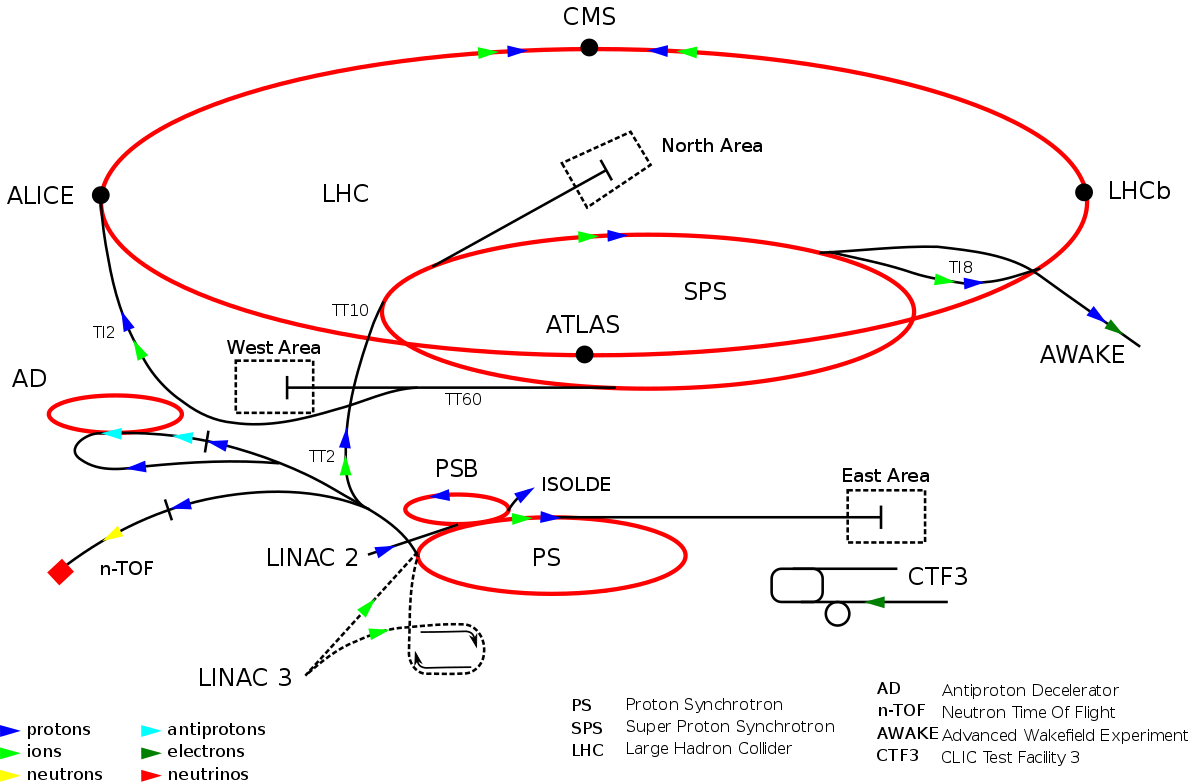
\includegraphics[width=0.9\textwidth]{fig/lhc/LHC_complex.png}
\caption{\label{fig:LHC_complex} The CERN accelerator complex. The proton injection chain for the LHC starts from the LINAC2 and proceeds through the Booster, PS, and SPS.}
\end{figure}

The performance of an accelerator is measured in terms of instantaneous luminosity $\mathcal{L}$; the most important characteristic of a collider is that it ties the event rate to the cross-section ($\sigma$) of a process:
\begin{equation}
\frac{dN_{i}}{dt} = \sigma_{i} \mathcal{L}(t)
\end{equation}
Where $i$ indicates any general process and $\mathcal{L}(t)$ is the instantaneous luminosity that depends on the number of interactions per unit of time. The machine’s instantaneous luminosity is related to the parameters of the beam and can be written as follows:
\begin{equation}
\mathcal{L} = \frac{f_{rel}N_{b}^{2}n_{b}\gamma_{r}}{4\pi\epsilon_{n}\beta^{\ast}}F
\end{equation}
Where $f_{rev}$ = 11\,kHz is the revolution frequency; $N_{b}$ is the number of particles per bunch; $n_{b}$ is the number of bunches per beam; $\epsilon_{n}$ is the normalized transverse beam emittance; $\beta^{\ast}$ is the beta function at the collision point, which measures the beam focalization and is corrected by the relativistic gamma factor $\gamma_{r}$; and F is a geometric luminosity reduction factor that accounts for the crossing angle at the interaction point~\cite{lumi_formula}. The amount of data delivered by a collider is measured in terms of the total integrated luminosity, $L = \int\mathcal{L}dt$, and measured in unit fb$^{-1}$. Since discoveries in particle physics depend on statistics, the higher the luminosity, the more chances physicists of discovering a particle or process.

During 2016, the LHC was running at centre-of-mass energy $\sqrt{s} = 13$\,TeV with a bunch spacing of 25\,ns. Reducing $\beta^{\ast}$ parameter from 80\,cm to 40\,cm, the nominal LHC luminosity crossed the record value of $10^{34}$\,cm$^{-2}$\,s$^{-1}$ in late summer 2016. The instantaneous luminosity delivered by LHC (blue) and recorded by CMS (yellow) is shown in Fig.~\ref{fig:cms_lumi}(a) and the total integrated luminosity during 2016 in Fig.~\ref{fig:cms_lumi}(b).   


\begin{figure}[htp]
\centering
\begin{tabular}{cc}
\hspace{-0.3cm}
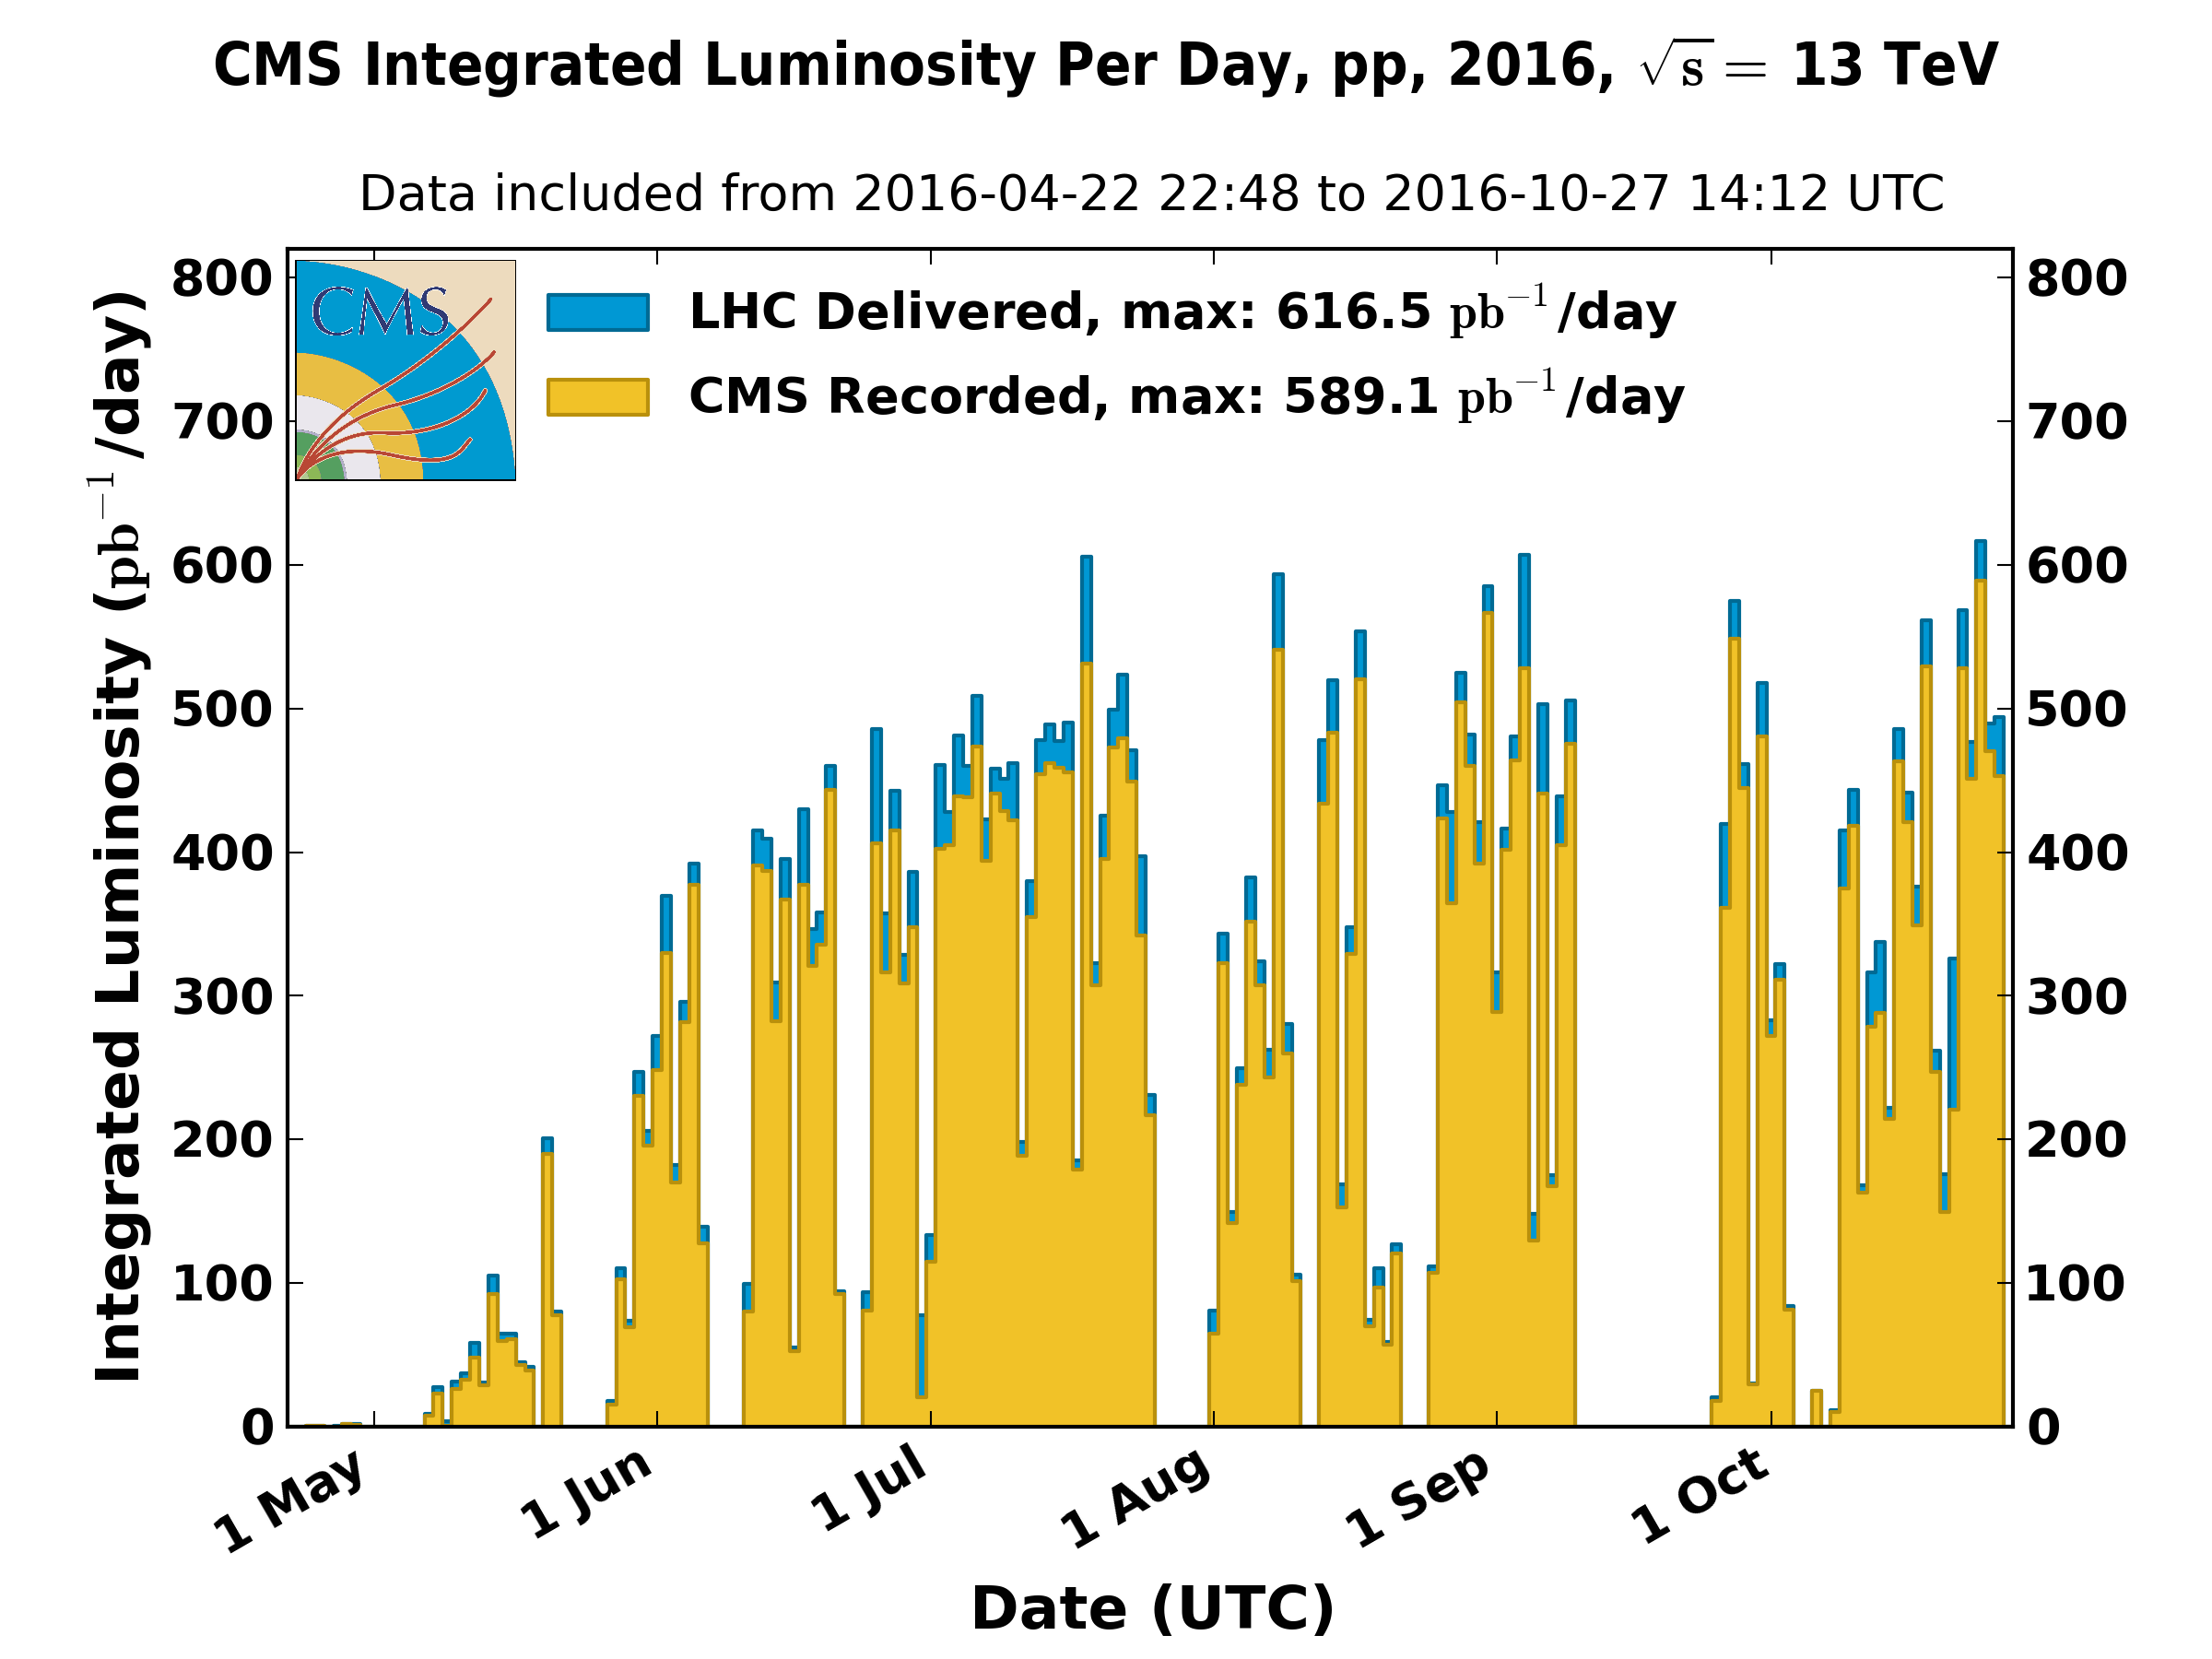
\includegraphics[scale=0.39]{fig/lhc/int_lumi_per_day_pp_2016.png}
& \hspace{-0.5cm} 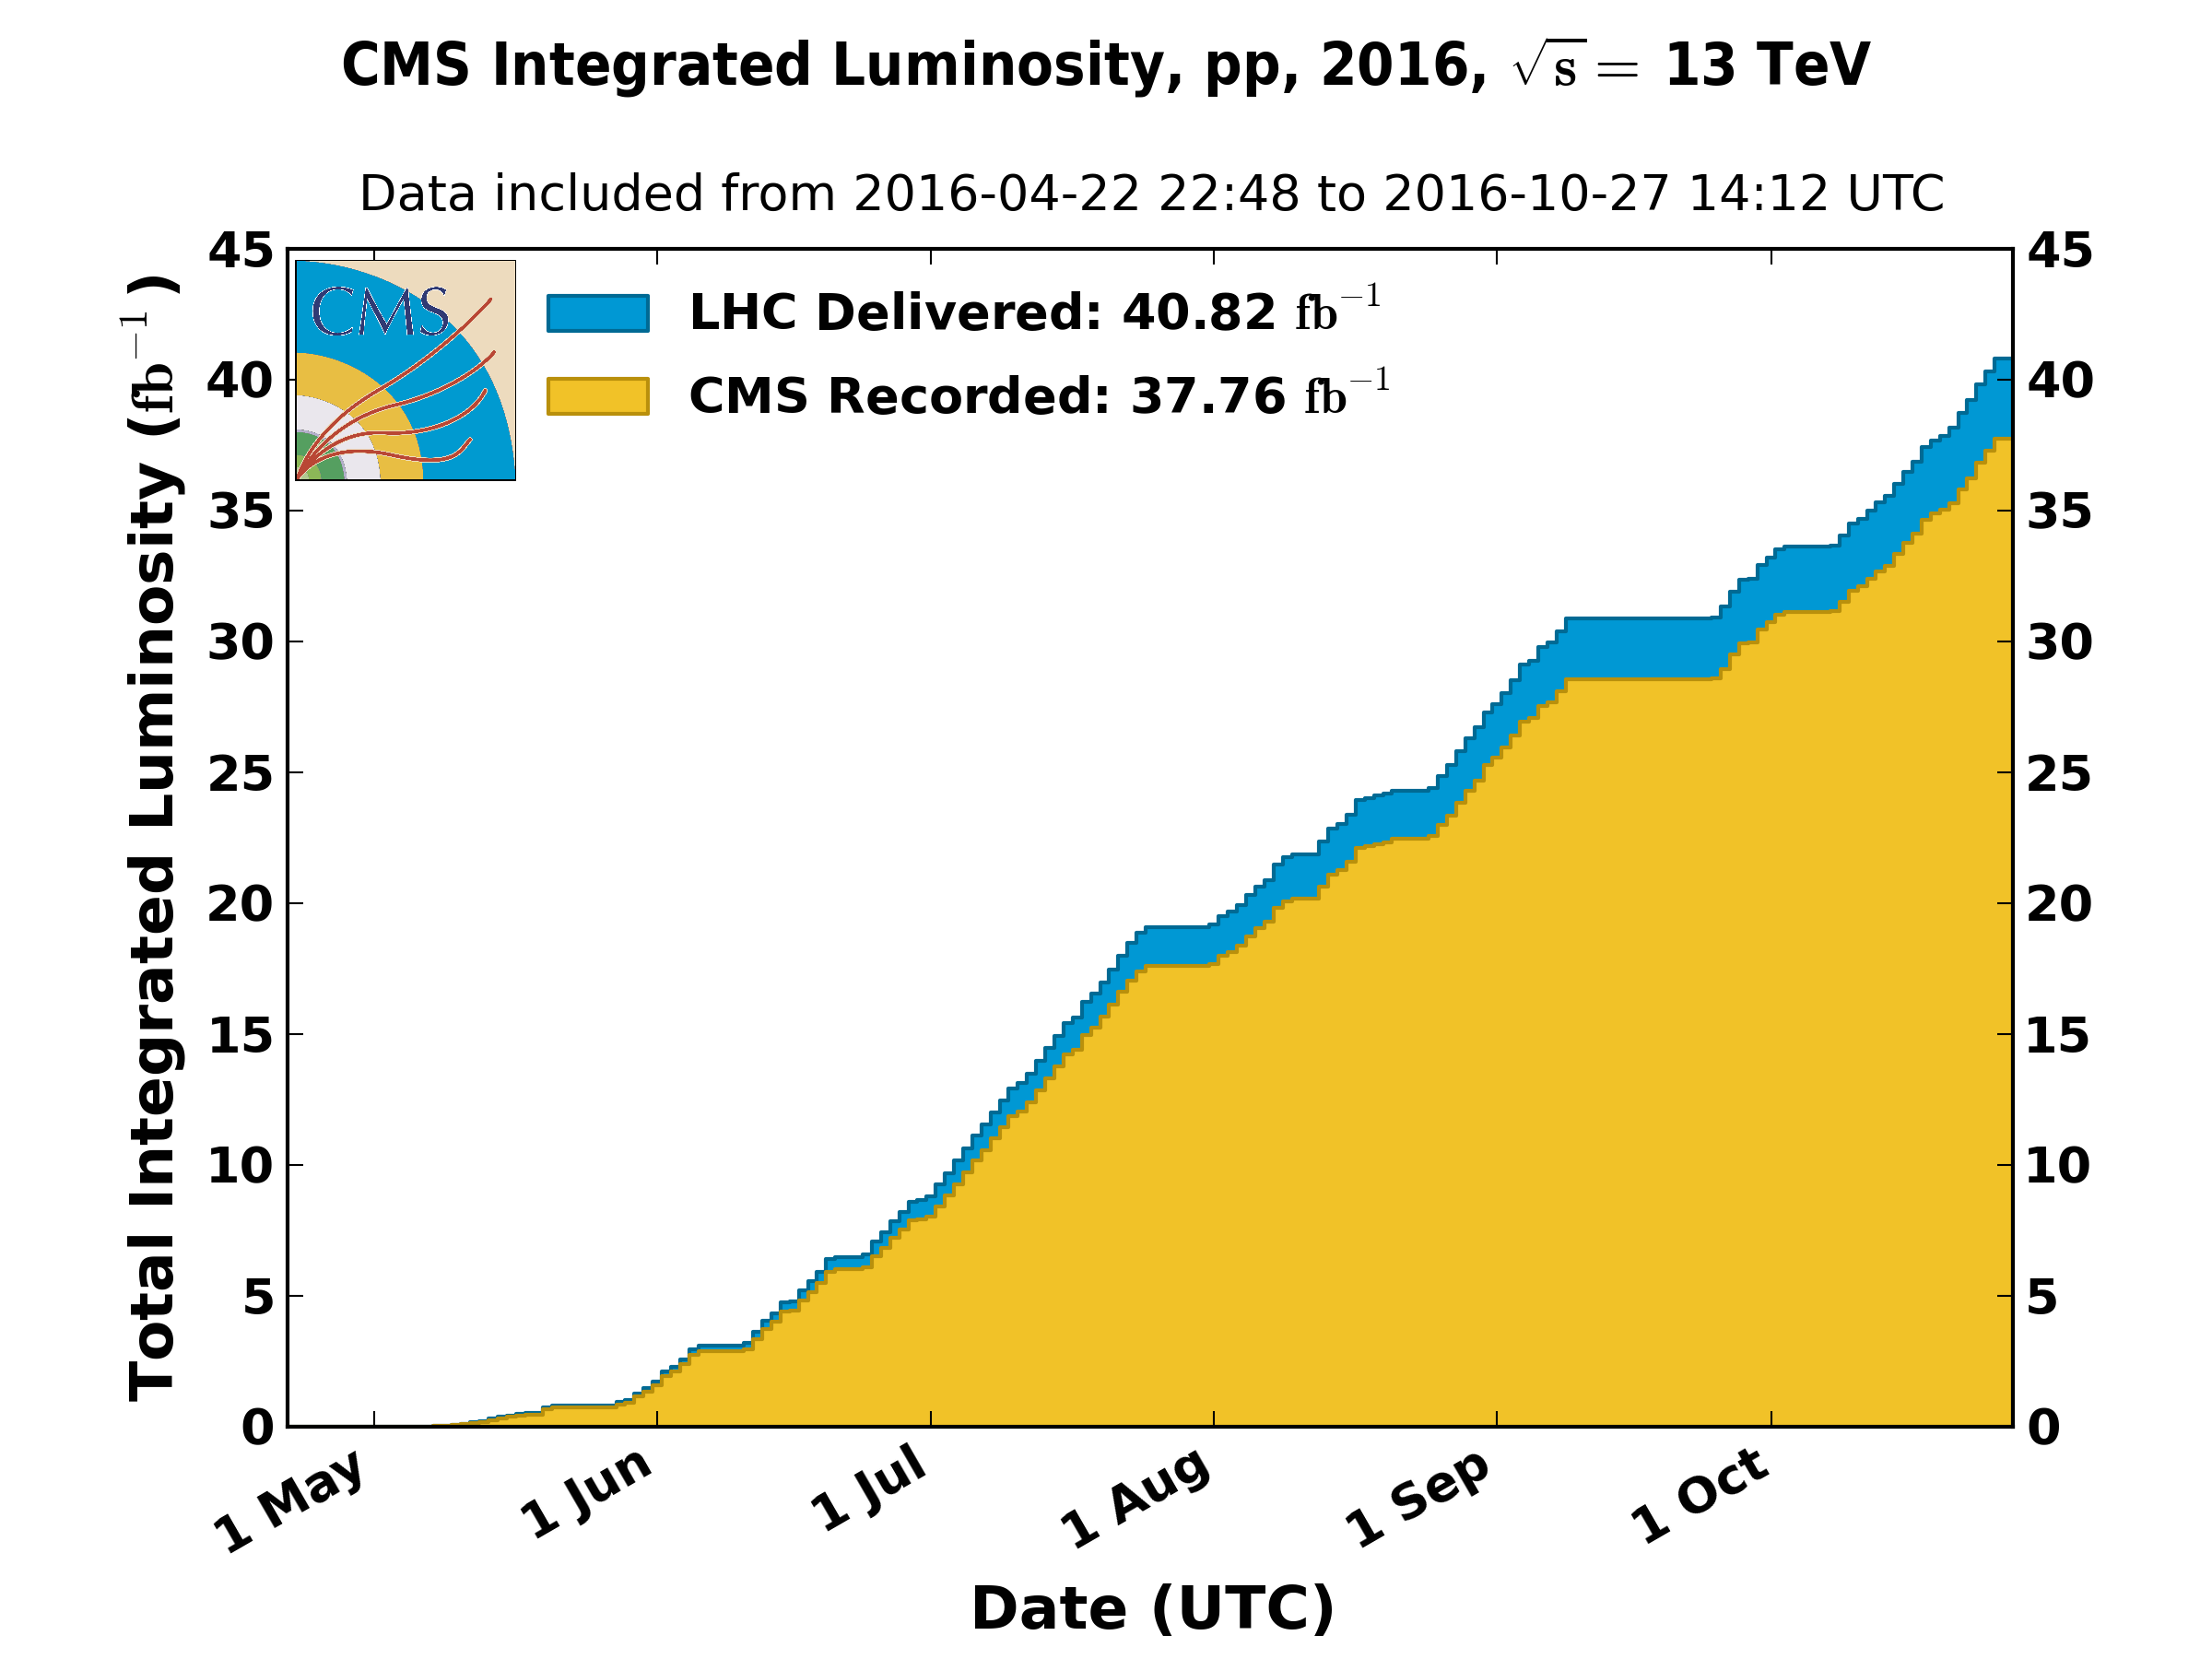
\includegraphics[scale=0.39]{fig/lhc/int_lumi_per_day_cumulative_pp_2016.png}\\
   ($\mathbf{a}$)\qquad&($\mathbf{b}$)\qquad\\
\end{tabular}
\caption{The evolution of the instantaneous luminosity per day (a) and the integrated luminosity (b) delivered by LHC (blue) and recorded by CMS (yellow) in 2016. The plots have been taken from~\cite{twiki:cms_lumi}.}\label{fig:cms_lumi}
\end{figure}

Among the four detectors, two (ATLAS (A Toroidal LHC ApparatuS) and CMS (Compact Muon Solenoid)) are the largest multi-purpose experiments. Their main focus is the precise measurements of SM and BSM physics. ALICE (A Large Ion Collider Experiment) is designed for heavy-ion collisions to study the physics of strongly interacting matter at extreme energy densities as well as the quark-gluon plasma. The Hadron Collider beauty (LHCb) experiment is designed to study heavy flavour beauty hadron physics.

\section{The CMS experiment at the LHC}\label{sec:cms}
The CMS~\cite{cms_exp} is one of the two multi-purpose experiments installed at the LHC ring to study a wide range of particles and heavy-ion physics. The primary goals are to elucidate the nature of the electroweak symmetry breaking mechanism linked to the Higgs mechanism, search for physics Beyond the Standard Model (BSM), and obtain precise measurements of various SM processes. An overview of the CMS detector and its subsystems is shown in Fig.~\ref{fig:CMS_exper}. The general concept driving the detector design is the configuration of the magnetic field needed to bend the trajectory of the charged particles, especially muons, to have a good resolution while measuring high momentum. The CMS detector has a superconducting solenoid magnetic producing a field of 3.8\,T parallel to the beam axis, encapsulating a high-quality tracking system and calorimeters. The muon system is installed outside the magnet in four stations and interleaved with return yoke. The magnetic field is strong enough to saturate 1.5\,m of iron. Each muon station consists of several layers of aluminium drift tubes (DT) in the barrel region (coaxial to the beam axis) and cathode strip chambers (CSCs) in the endcap region (perpendicular to the beam axis), complemented by resistive plate chambers (RPCs). The CMS detector is relatively compact in spite of its heavy weight, 12,500\,Tons (as compared to ATLAS), with a length of 21.6\,m and a diameter of 14.6\,m.  

\begin{figure}[h!]
%\centering
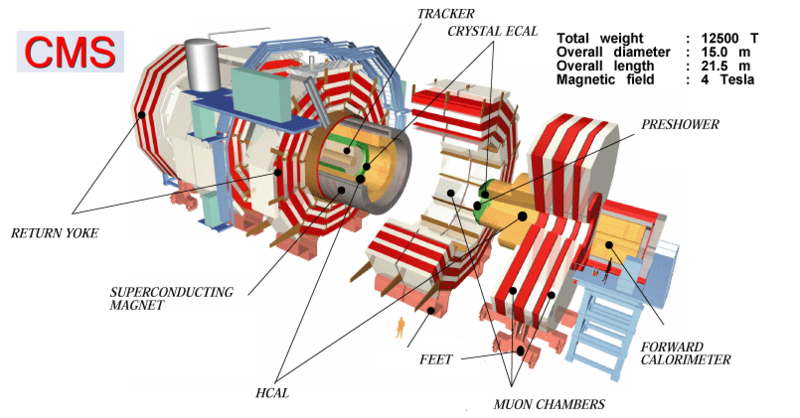
\includegraphics[width=1.05\textwidth]{fig/lhc/CMS_exper.png}
%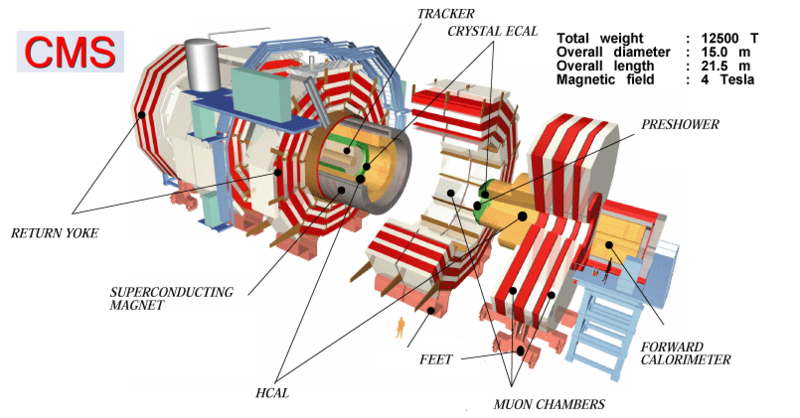
\includegraphics[scale=0.4, trim=20 50 60 30,clip]{fig/lhc/CMS_exper.png}
\caption{\label{fig:CMS_exper} An overview of the CMS detector showing the major sub detectors.}
\end{figure}
The CMS experiment adopted a cylindrical coordinate system with its origin at the nominal interaction point at the centre of the detector. The z-axis is chosen along the anti-clockwise beam and is referred to as longitudinal. The x-axis points radially towards the centre of the LHC ring, and the y-axis is vertical and points upwards as shown in Fig~\ref{fig:CMS_coordinates}. 
\begin{figure}[h!]
\centering
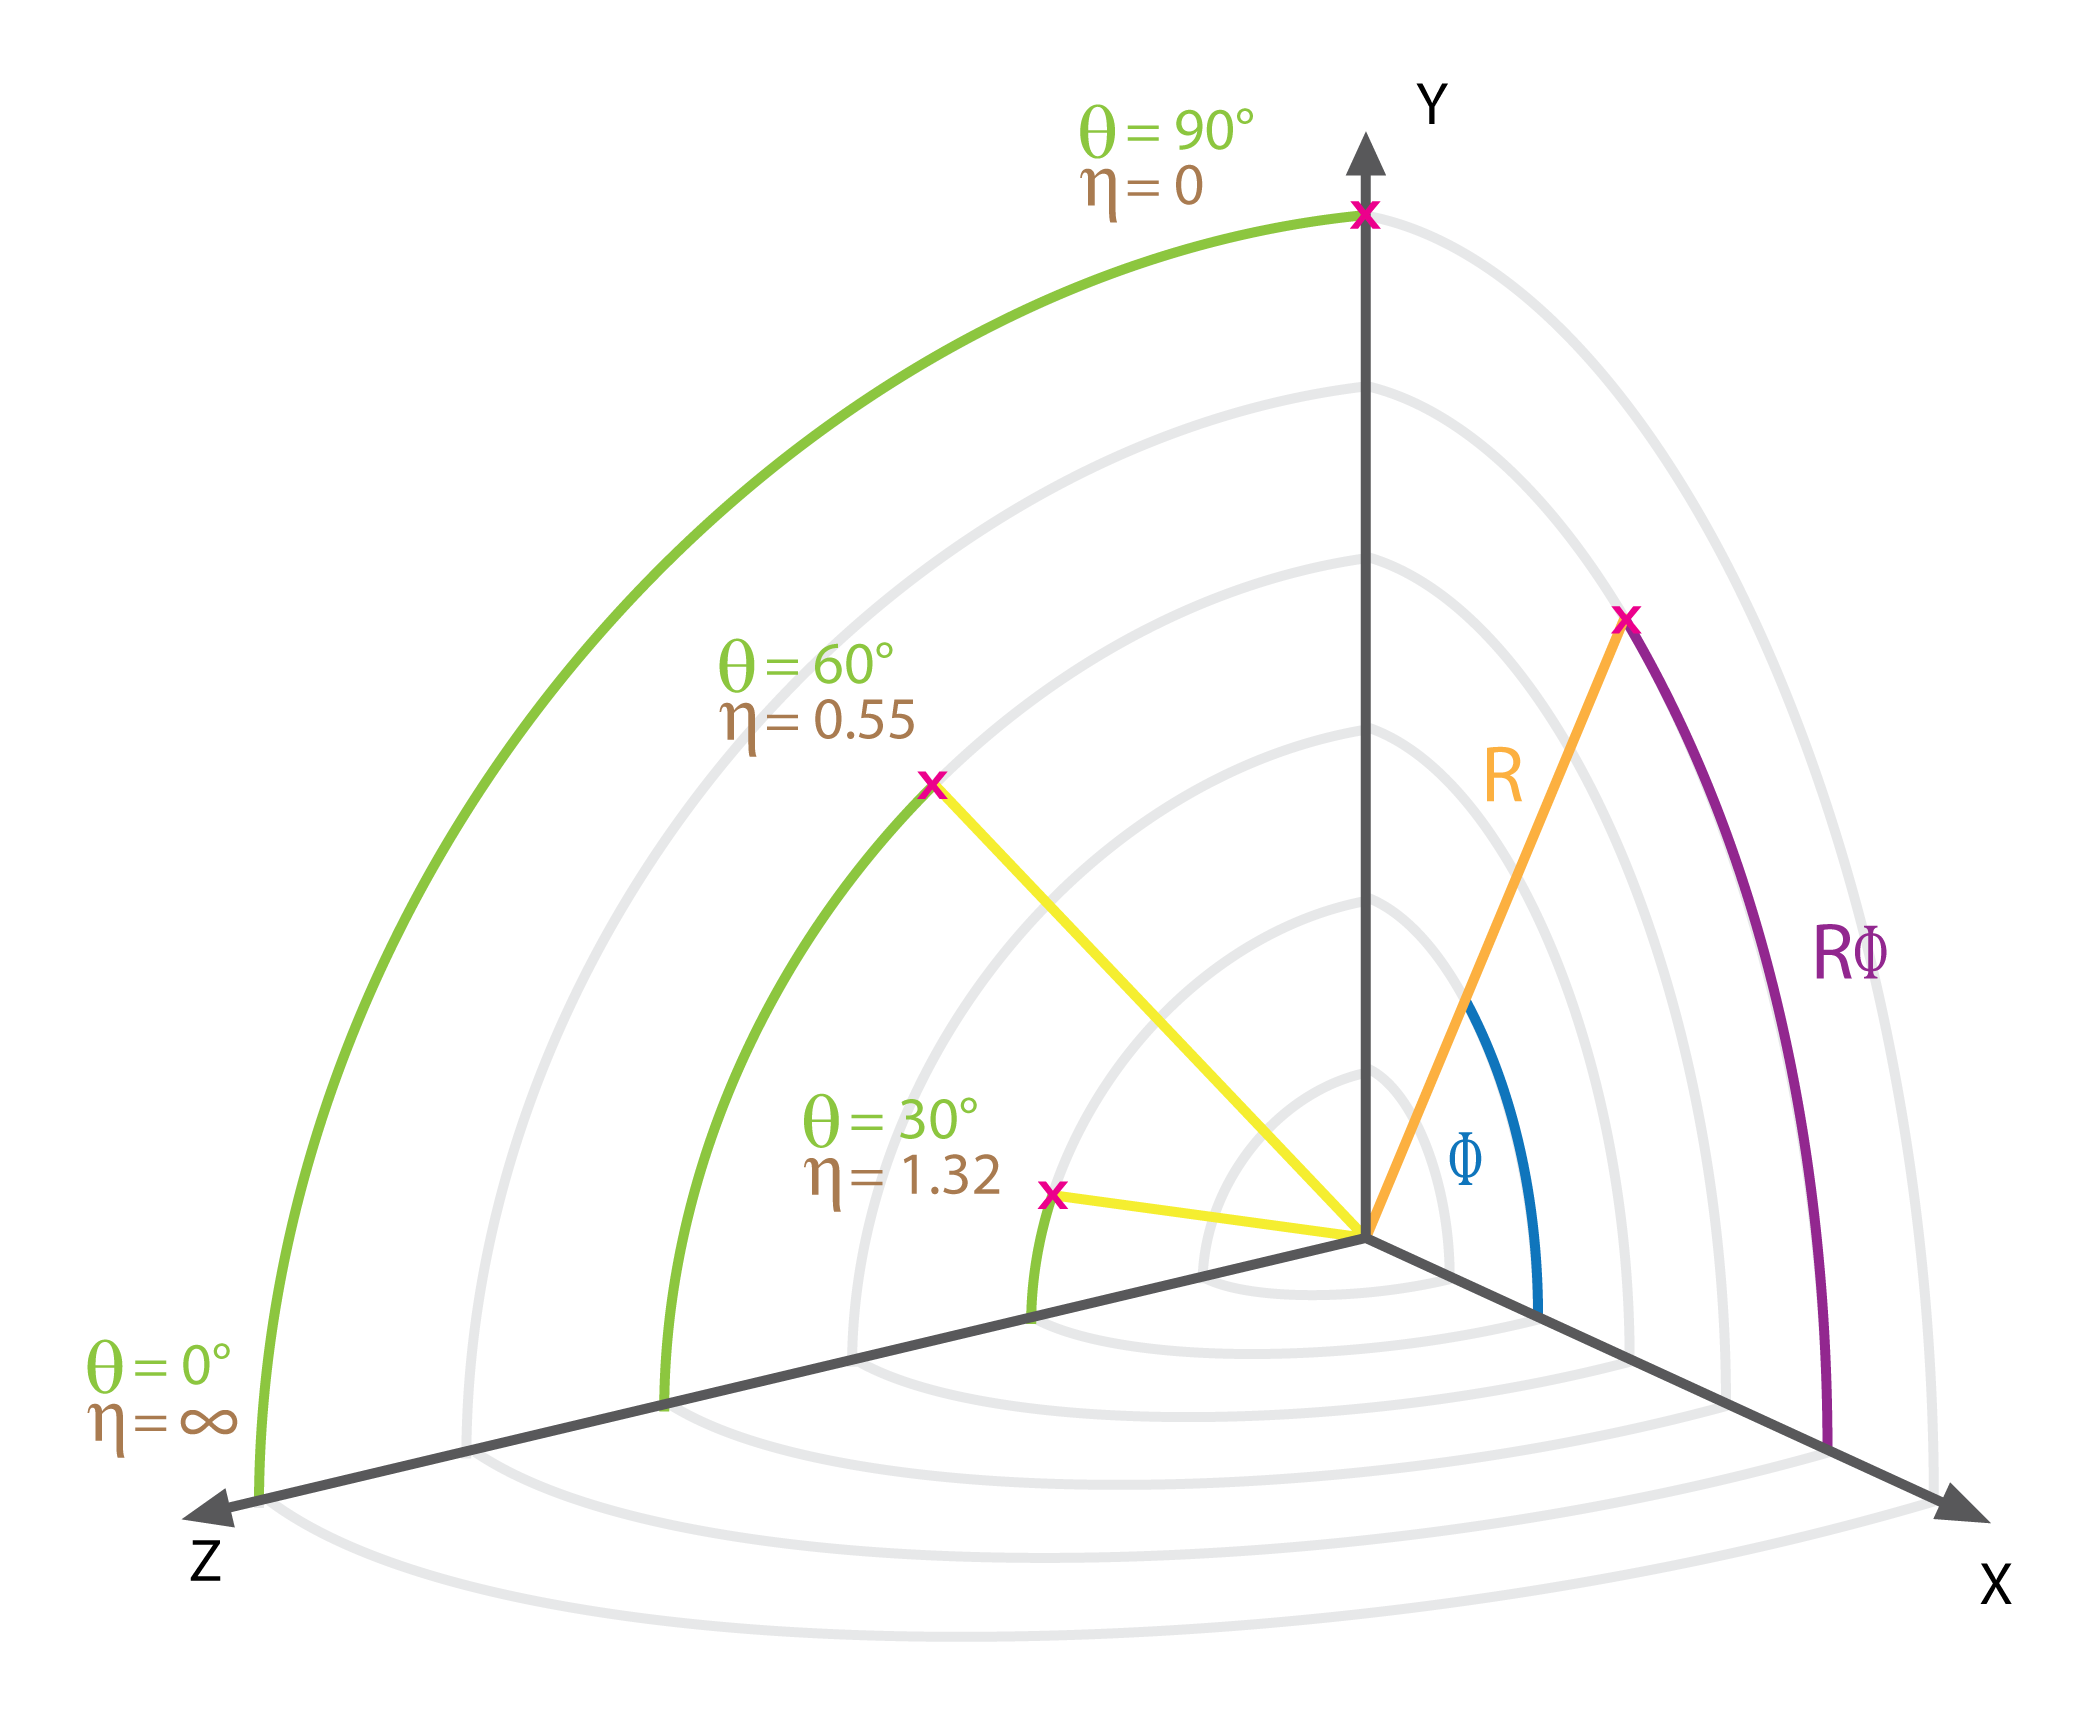
\includegraphics[width=0.6\textwidth]{fig/lhc/img_cms_coordinates.png}
\caption{\label{fig:CMS_coordinates} An overview of the CMS experiment coordinate system.}
\end{figure}
The azimuthal angle $\phi$ is measured on the x-axis in the x-y plane, where the x-y plane is perpendicular to the beam axis and called the transverse plane. The polar angle $\theta$ is measured on the z-axis. Instead of $\theta$, the angular position is preferentially expressed in terms of a kinematic quantity called pseudorapidity ($\eta$), defined as:
\begin{equation}
\eta \equiv -ln(tan(\frac{\theta}{2}))
\end{equation}
Adopting the above coordinate system, a particle momentum $p$ has two components, one transverse to the beam direction denoted by $p_{T}$ and calculated using the x and y components. The second component is the longitudinal one, $p_{z}$, pointing along the z-axis. The missing transverse energy $E_{T}^{miss}$ term is used for imbalance in total transverse energy of a collision. The angular separation between the two particles is usually expressed in the $\phi-\eta$ plane, expressed as:
\begin{equation}
\Delta R = \sqrt{\Delta\Phi^{2} + \Delta\eta^{2}}
\end{equation} 
In the following section, a brief summary of all the subsystems of the CMS experiment is given.

%================================================
\subsection{Tracker}
The tracker is the innermost and closest to the interaction point, sub-detector of CMS, immersed in the homogeneous magnetic field of 3.8\,T provided by the solenoid. It is designed to measure the momentum and charge of charged particles emerging from the interaction point by determining the bending of their trajectories in their passage through the detector layers. Secondary vertices can also be reconstructed in association to the late decays of particles such as B hadrons. The trajectory deviation from the straight-line propagation is measured by the sagitta:
\begin{equation}
s \approx \frac{0.3BL^{2}}{8p_{T}}
\end{equation}
Where $s$ is sagitta, $B$ is the solenoid magnetic field, $L$ is the track length, and $p_{T}$ is the transverse momentum. The transverse momentum resolution is mainly dependent on the geometric accuracy on the sagitta ($\sigma_{s}$) using:
\begin{equation}
\frac{\sigma_{p_{T}}}{p_{T}} \approx \frac{8p_{T}}{0.3BL^{2}}.\sigma_{s}
\end{equation}
At the LHC, design luminosity and energy (around 1\,MHz/mm$^{2}$ at 4\,cm from the beamline), several hundred particles go through the tracker during each bunch crossing; high granularity, fast response, and high-radiation tolerance are especially important to its design. In order to fulfil the aforementioned criteria, the semiconductor silicon technology was chosen to build the inner tracking system~\cite{tracker}. Charged particles traversing a sensor produce electron-hole pairs that drift under an applied electric field, giving rise to a current pulse. Cooling is ensured by liquid perfluorohexane that maintains the sensor temperature at around \SI{-10}{\celsius} to limit the noise due to radiation-induced leakage.

The tracker occupies a cylindrical volume of 5.8\,m in length and 2.5\,m in diameter with a surface area of 210\,m$^{2}$, extends in the region of $\abs{\eta}$ < 2.5, r < 120\,cm, $\abs{z}$ < 270\,cm. A schematic view of the CMS tracker is shown in Fig.~\ref{fig:tracker}. 

\begin{figure}[h!]
\centering
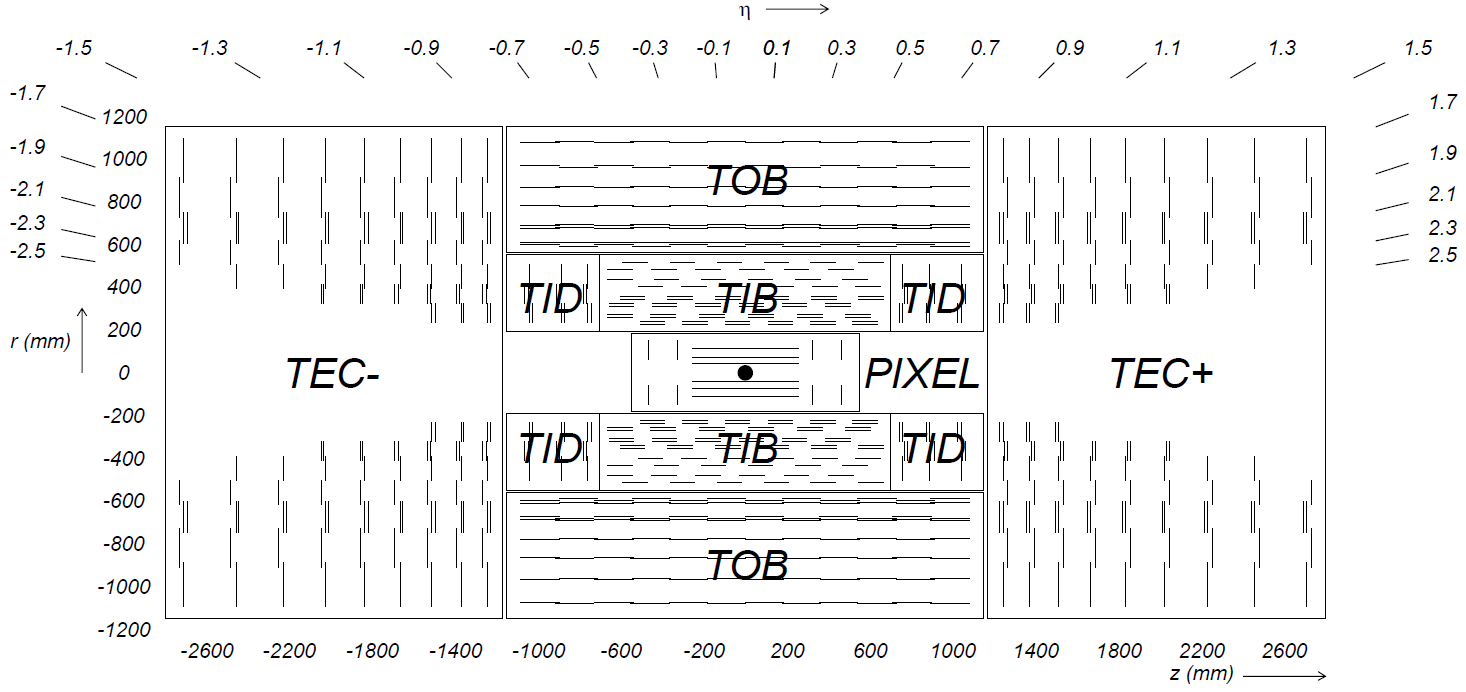
\includegraphics[scale=0.3]{fig/lhc/Tracker.png}
\caption{\label{fig:tracker} The CMS tracker system with its subsystems in the (r, z) plane.}
\end{figure}
The tracker has two sensors classes – pixel and strip detectors.
\begin{itemize}
\item{\textbf{Pixel Tracker System:}} is placed closest to the interaction point (r $\leq$ 10\,cm) because it has the largest track density. It is comprised of a total of approximately 66-million pixel cells grouped in 1440 modules with a cell size of 100 $\times$ 150 $\mu$\,m$^{2}$. They are arranged in three cylindrical barrel layers with a radii between 4.4\,cm and 10.2\,cm from the beam line and two endcap discs at each side of the barrel, approximately 34.5\,cm and 46.5\,cm from the interaction point. With a high reconstruction hit efficiency well above 99\%, the pixel detector covers a pseudorapidity range $\abs{\eta}$ < 2.5, corresponding to the acceptance of the entire tracker. The typical spatial hit resolution is measured to be around 10\,$\mu$m in the $r-\phi$ plane and 15\,$\mu$m along the z-axis, while the third coordinate is given by the sensor plane position, allowing for a three-dimensional vertex reconstruction.
\item{\textbf{Strip Tracker System:}} occupies the outer part of the tracker cope with reduced particle density. The silicon strip detector is made of two concentric sets of layers in the barrel (tracker inner barrel, TIB, and tracker outer barrel, TOB) occupying the region 20\,cm < $\abs{r}$ < 55\,cm and $\abs{z}$ < 118\,cm and two blocks of forward disks in the endcaps, called tracker endcaps (TEC) and tracker inner disk (TID) covering the region with 55\,cm < $\abs{r}$ < 116\,cm and $\abs{z}$ < 118\,cm. The single-point resolution is about 30\,$\mu$m in the $r-\phi$ plane and 300\,$\mu$m in the z direction.
\end{itemize} 

%================================================
\subsection{Electromagnetic calorimeter (ECAL)}
The CMS Electromagnetic Calorimeter (ECAL)~\cite{ecal} is a hermetic, homogeneous, and high-granularity system made of inorganic scintillating crystals. ECAL precisely measures the position and energy of electrons and photons, inducing electromagnetic showers in the material. The physical process that drives the design of the ECAL is the low-mass Higgs decay into two photons – $H \rightarrow \gamma\gamma$ – one of the leading channels for the study of the Higgs properties. ECAL provides excellent energy resolution in order to maintain the advantage of a narrow width in the low Higgs mass range. Its role in the $H \rightarrow ZZ \rightarrow 4l$ channel is also important with regard to reconstructing the electron along with the tracker. ECAL crystals are made of lead tungstate (PbWO$_{4}$) scintillating crystals that act both as absorbers with a short radiation length (X$_{0}$ = 0.89\,cm) and as scintillators with a very fast response (80\% of the light being emitted within 25\,ns), which deal with the LHC bunch spacing. Avalanche Photodiodes (APD) are used in barrel and Vacuum Phototriodes (VPT) in endcaps to detect scintillation light with wavelengths around 420\,nm. An overview of the CMS ECAL is shown in Fig.~\ref{fig:ecal}.
\begin{figure}[h]
\centering
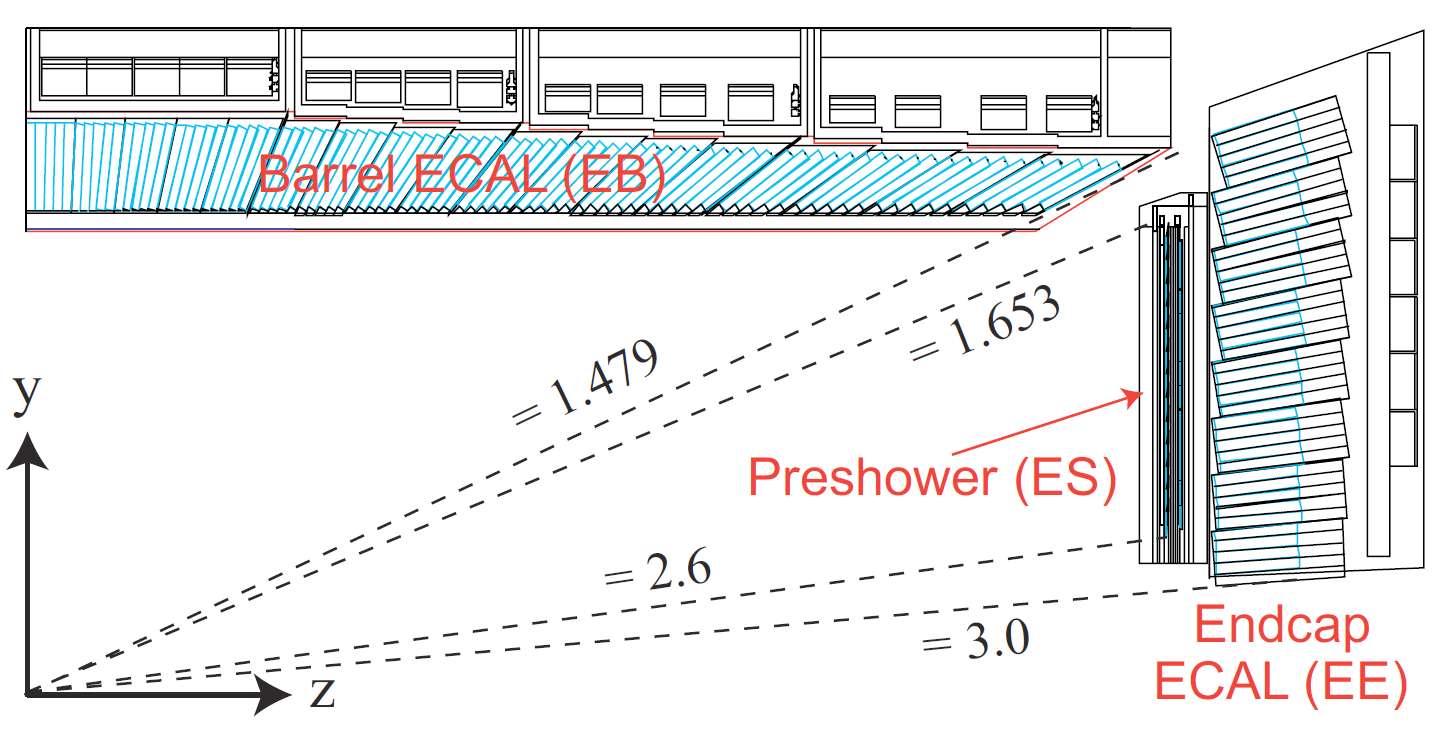
\includegraphics[scale=0.3]{fig/lhc/img_ECALRapidity.png}
\caption{\label{fig:ecal} The ECAL longitudinal overview of a quadrant.}
\end{figure}
\begin{itemize}
\item{\textbf{ECAL Barrel (EB):}} is located at a distance r = 129\,cm from the beam axis and covers a pseudorapidity range of 0 < $\abs{\eta}$ < 1.48. It is equipped with 61,200 crystals with a high granularity of 0.0174 $\times$ 0.0174\,rad in $\eta-\phi$ plane, each with a transverse section of 22 $\times$ 22\,mm$^{2}$ at the front face and a length of 230\,mm (25.8X$_{0}$). Crystals are grouped in arrays of 2 $\times$ 5, contained in a very thin 200\,$\mu$m alveolar structure, each corresponding to a sub-module. A group of 40/50 sub-modules are further assembled in modules, where four modules make a super-module. Finally, EB is divided into 36 super-modules, each subtending an angle of \ang{20} in $\phi$. 
\item{\textbf{ECAL Endcaps (EE):}} is located at a distance of $\abs{z}$ = 315.4\,cm from the interaction point and covers a range of 1.479 < $\abs{\eta}$ < 3 with identically shaped crystals, grouped in a carbon-fiber structure of 5 $\times$ 5 elements, called a super-crystal. The crystals have a rear face cross section of 30 $\times$ 30\,mm$^{2}$, a front face cross section of 28.62 $\times$ 28.62\,mm$^{2}$ and a radiation length of 220\,mm (24.7X$_{0}$). Each EE has 134 identical supercrystals with a further 18 sectioned supercrystals to complete the inner and outer perimeter.
\item{\textbf{ECAL Preshawer (ES):}} detectors are placed at each end of tracker, in front of EE and cover a pseudorapidity range 1.653 < $\abs{\eta}$ < 2.6. It is a two-layer sampling calorimeter consisting of lead radiator layer with a total of 3X$_{0}$ that initiates electromagnetic showers from incoming particles, and silicon strip sensors that measure the deposited energy and transverse shower profiles. The ES help distinguish $H \rightarrow \gamma\gamma$ decays from single photons, and to identify electrons against minimum ionizing particles.
\end{itemize}
Energy resolution of ECAL for energies below than 500\,GeV is given by:
\begin{equation}
(\frac{\sigma_{E}}{E})^{2} = (\frac{S}{\sqrt{E}})^{2} + (\frac{N}{E})^{2} + C^{2}
\end{equation}
where $S$ is the stochastic term arising due to fluctuations in the lateral shower containment, photostatistics and preshower energy deposition, the second term quantifies the effect of electronic noise and pile-up and a constant term is related to the non-uniformity of longitudinal light collection, calibration uncertainties and energy leakage from the back. ECAL barrel module's performance is studied using the test-beam data, typical values obtained are S = 2.8\%, N = 12\% and C = 0.30\%~\cite{ecal_resol};

\subsection{Hadronic calorimeter (HCAL)}
The CMS hadronic calorimeter (HCAL)~\cite{hcal} is a hermetic sampling calorimeter which measures precisely the energy and position of charged and neutral hadrons in the form of jets. It also provides an indirect measurement to non-interacting particles in terms of missing energy ($E_{T}^{miss}$). HCAL surrounds the ECAL and the design is restricted by geometrical dimensions of the ECAL and magnet systems. A schematic overview of the HCAL is shown in Fig~\ref{fig:hcal} with its four sub-detectors.
\begin{figure}[h!]
\centering
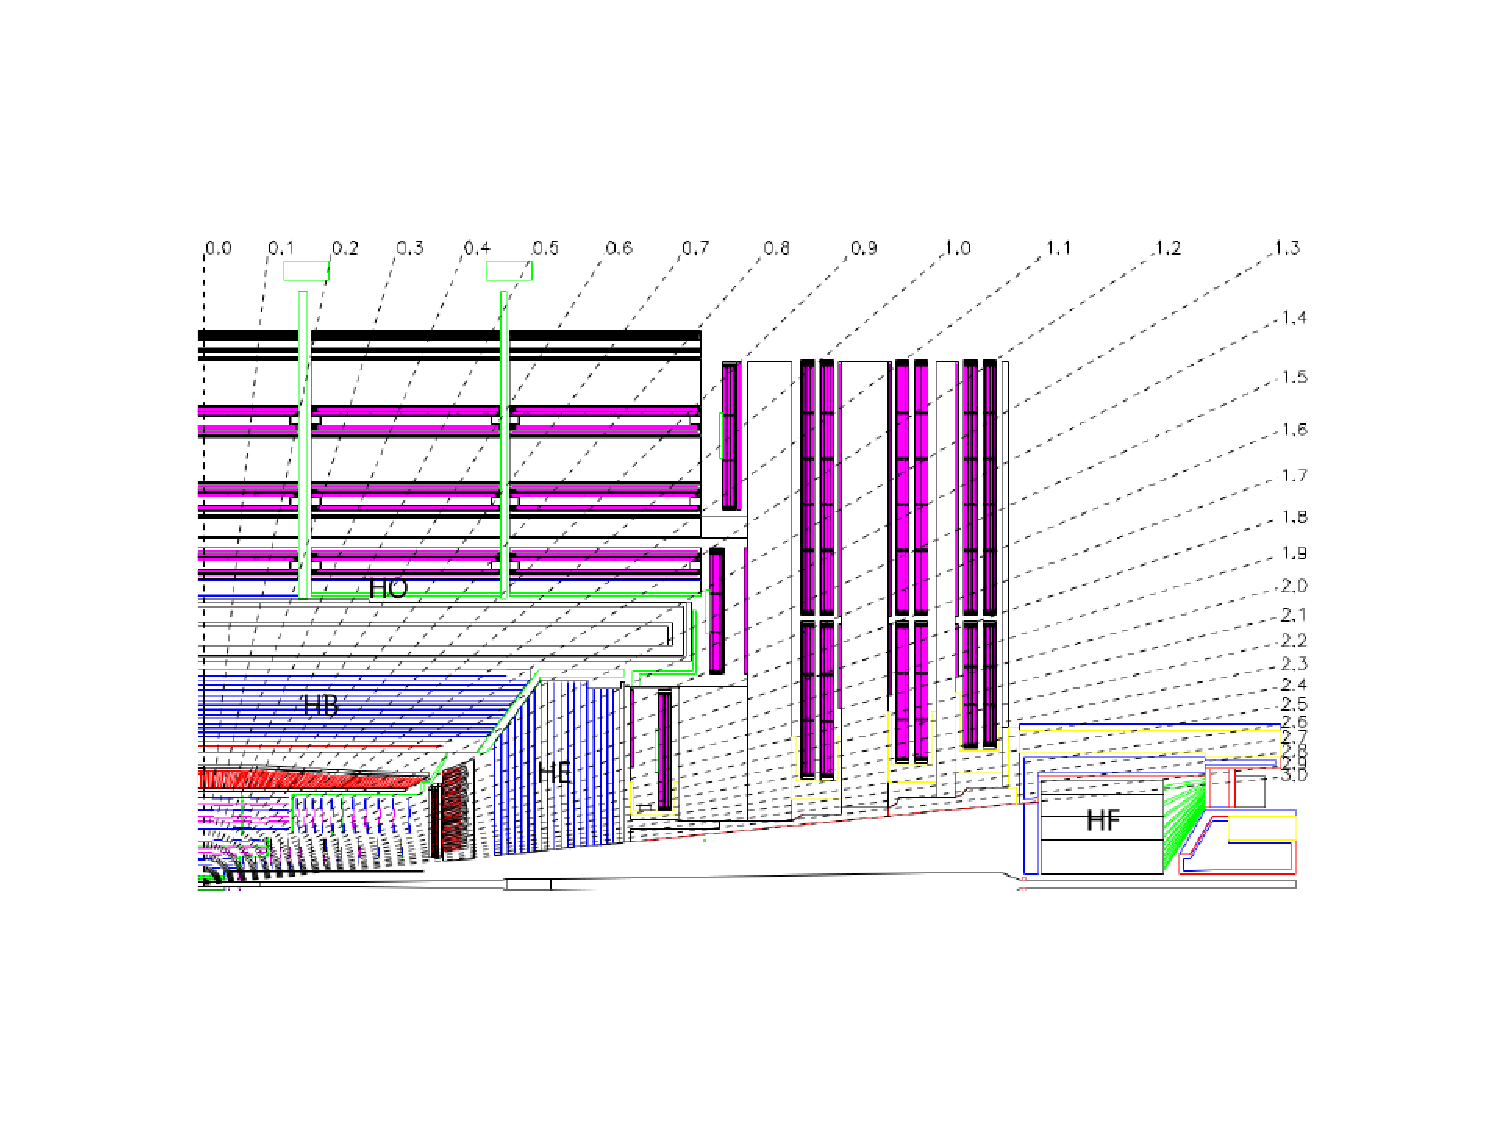
\includegraphics[scale=0.8, trim=90 100 80 80,clip]{fig/lhc/HCAL.pdf}
\caption{\label{fig:hcal} Longitudinal overview of the one quadrant of the CMS HCAL.}
\end{figure}
The HCAL Barrel (HB) comprise of two half-barrel sections covering a total pseudorapidity range of $\abs{\eta}$ < 1.3, located between EB with r = 1.77\,m and the inner extent of the magnet coil (r = 2.95\,m), corresponds to interaction lengths of 5.82\,$\Lambda_{I}$ in the central region. Due to space restriction, the HB is complemented by an additional layer of scintillators outside the solenoid, referred to as the Hadronic Outer (HO) calorimeter. HO provides additional depth up to a minimum 11.8\,$\Lambda_{I}$ to the HCAL system in the radial direction and have same characteristics as HB. 

The HCAL Endcap (HE) covers forward region in pseudorapidity range of 1.3 < $\abs{\eta}$ < 3.0 and has sufficient depth around 10\,$\Lambda_{I}$. HB and HE use non-magnetic brass layers as absorber material, and are interspersed with plastic scintillator tiles which serve as the active medium. Two forward hadron calorimeters (HF) are installed which cover the very forward region in pseudorapidity given by 3.0 < $\abs{\eta}$ < 5.0, positioned at $\abs{z}$ = 11.2\,m from the interaction point, thus ensuring good hermeticity. HF detectors using steel as absorber and Cherenkov-light-emitting quartz fibres are as active medium, motivated by the high particle flux in this region. The energy resolution of the HCAL system can be expressed in stochastic term $a$ and constant term $b$ as:
\begin{equation}
(\frac{\sigma_{E}}{E})^{2} = (\frac{a}{\sqrt{E}})^{2} + b^{2}
\end{equation}
%=========================================================
\subsection{Magnet}
The CMS detector uses solenoidal magnetic field which is the core of detector and hence the name of experiment. A strong magnetic field is needed to achieve good resolution of the high momentum charged particle up to 1\,TeV by measuring curvature while direction gives charge of particle~\cite{cms_magnet}. The structure of superconducting magnet for CMS  has 6\,m diameter and 12.5\,m length, able to generate a uniform magnetic field of 3.8\,T with a stored energy of 2.3\,GJ at full current of 19500\,A. A graphical overview of the CMS magnetic field is shown in Fig.~\ref{fig:magnet}. The magnet mainly uses a superconducting coil (ensured by a helium cooling system at temperature 4\,K), a vacuum tank (responsible to isolate it from the external environment) and a 10000 ton magnet yoke comprising five wheels and two endcaps (necessary to return magnetic flux, which otherwise would get lost, disturbing the surrounding environment). 
\begin{figure}[h]
\centering
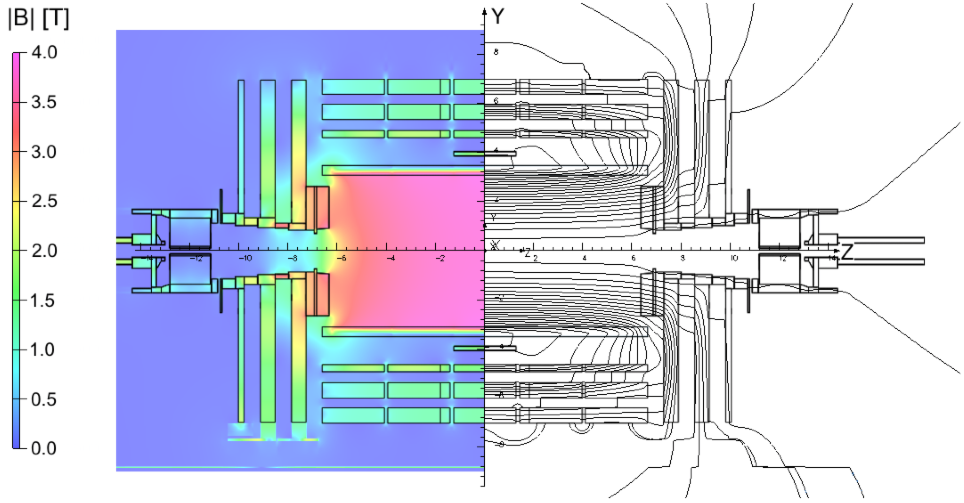
\includegraphics[scale=0.4]{fig/lhc/Sections_IntroductionFigs_MagField.png}
\caption{\label{fig:magnet} Longitudinal view of the CMS detector magnet where left side shows simulation of the magnetic field and the magnetic field lines are at the right side. At the heart of the detector, the magnetic field value is 3.8\,T.}
\end{figure}
%========================================
\subsection{Muon spectrometer}
Muon plays a key role in the search for many physics phenomena, ranging from precise measurement of the SM of particle physics to new searches, especially in the discovery of SM Higgs boson through golden channel ($H\rightarrow ZZ \rightarrow 4l$). Being a massive particle as compared to electrons, the muon is less effected by bremsstrahlung radiations and traverses through all sub detectors. Owing to these characteristics, the muon system is placed behind all the sub detectors. It is embedded in the return yoke of the solenoid. Muons bring a highly clean signature to the spectrometer because other particles are stopped by the calorimeters. The CMS muon spectrometer covers a pseudorapidity range to $\abs{\eta}$ < 2.4 and consists of three subsystems, Drift Tubes (DTs), Cathode Strips Chambers (CSCs), and Resistive Plate Chambers (RPCs)~\cite{cms_muon}, as shown in Fig.~\ref{fig:rpc_dt}.   

\begin{itemize}
\item{\textbf{Drift Tubes:}}
In the barrel region of the CMS detector, the magnetic field is mostly uniform and the muon rate is low. Four layers of muon stations are installed, consisting of drift tube (DTs) chambers covering a pseudorapidity region of $\abs{\eta}$ < 1.2. In each wheel, DTs are installed into 12 $\phi$-segments, forming four stations in the radial direction and interleaved between the plates of the return yoke. In the longitudinal (except MB4) and bending plane, each station consists of four and eight layers of DTs respectively to enable the precise measurement of position.

DTs consist of an individual cell with grounded walls acting as cathode and a 50\,$\mu$m-diameter gold-plated stainless-steel anode wire at the centre of the cell. The drift electric field is created by two electrode plates mounted at the two sides of the cell. The cells use a gas mixture of 85\% of Ar and 15\% CO$_{2}$ with HV settings: V$_{wire}$ = +3600V, V$_{cath}$ = -1800\,V and V$_{strip}$ = +1800V~\cite{muon-sys}.  
\item{\textbf{Cathode Strip Chambers:}}
Cathode Strip Chambers (CSCs) are installed in endcap regions of pseudorapidity coverage 0.9 < $\abs{\eta}$ < 2.4. Due to the higher muon flux, background radiation, and non-uniform magnetic field in the endcap region, CSC detectors are designed to be robust, fast, radiation hard, and finely segmented. CSCs operate as standard multi-wire proportional counters, comprising six planes of anode wires interleaved among seven cathode strips. The anode wires run azimuthally and identify the radial component of a track hit. The cathode strips are oriented radially, almost perpendicular to the wires and provide a precise measurement in the r-$\phi$ bending plane. The CSCs system uses a nominal gas mixture of 40\% Ar, 50\% CO$_{2}$ and 10\% CF$_{4}$.

\item{\textbf{Resistive Plate Chambers:}}
The muon system of the CMS experiment comprises of a third type of muon detectors, Resistive Plate Chambers (RPCs), installed both in the barrel and endcap regions along with DT and CSC, covering a pseudo rapidity range of $\abs{\eta}$ < 1.6. RPCs are gaseous parallel-plate detectors that operate in avalanche mode and are capable of tagging the time of an ionizing event in times less than 25\,ns (bunch crossing time at the design luminosity of the LHC). This makes RPCs an ideal trigger system that provides correct bunch-crossing time information between two successive bunches with muons, even at the largest LHC luminosities.
CMS RPC detector is a double-gap chamber where each gap separates two parallel plates of bakelite with a bulk resistivity of 10$^{10}$–10$^{11}$\,$\Omega$cm. A gas mixture of 95.2\% C$_{2}$H$_{2}$F$_{4}$, 4.5\% i-C$_{4}$H$_{10}$, and 0.3\% HF$_{6}$ is used in RPC operation, where C$_{2}$H$_{2}$F$_{4}$ is ionized by incident particles and the other two gases act as quenching agents, preventing the detector from streamer mode. The operational voltage of RPCs is lower than 10\,kV with an efficiency of about 100\%. 
\end{itemize}
\begin{figure}[h]
\centering
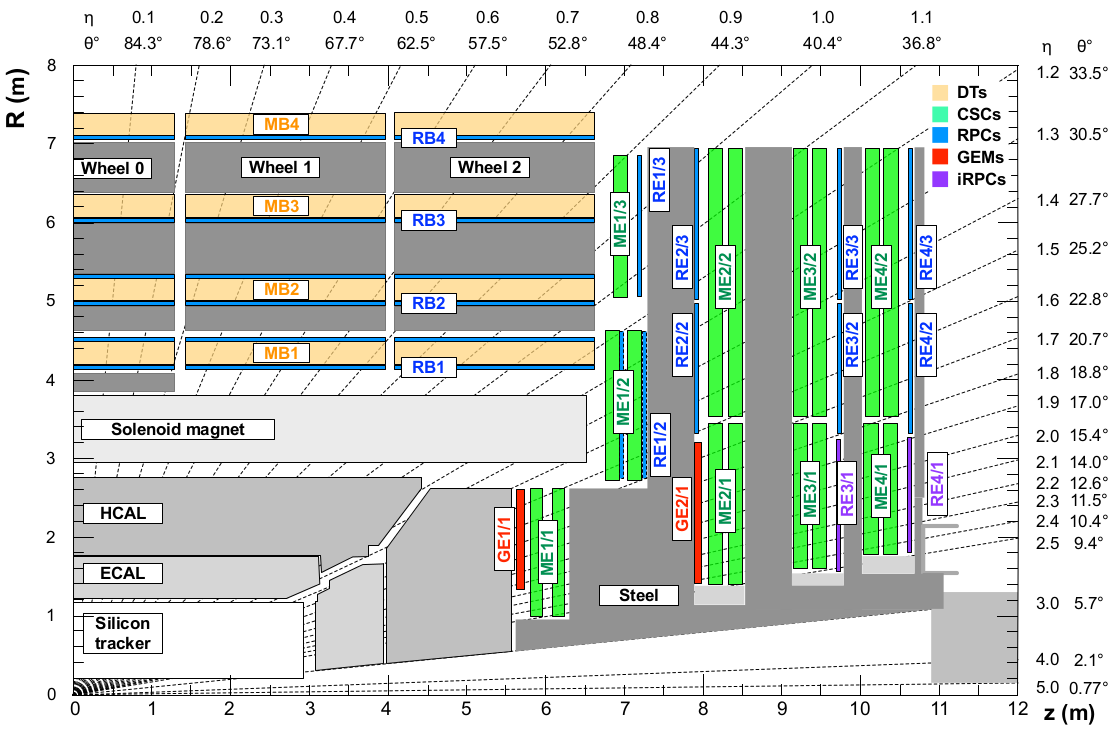
\includegraphics[scale=0.55]{fig/lhc/rpclayout.png}
\caption{\label{fig:rpc_dt} Quadrant of CMS muon system in (R, z) plane, where R is perpendicular to the beam axis and z is the distance in meters along beam axis. DTs are shown using light oranges, CSCs by green, and RPCs by blue.}
\end{figure}

%==============================
\subsection{Trigger and data acquisition systems}
The protons in the LHC beam are 25\,ns apart, which corresponds to 40\,MHz. On an average, there are 20 proton-proton collisions per bunch crossing. This produces an enormous amount of data, and the average size of an LHC event is around 1\,MB. Due to the limitations of detector performance and storage system, the event rate needs to be reduced to few hundred events per second. The CMS experiment uses a dedicated two-level (Level-1 and HLT) trigger system to control the event rate~\cite{cms_trigger}.

\textbf{L1 Trigger}: A hardware-based trigger system that reduces the event rate to 100\,kHz with a maximum decision time of 4\,$\mu$s per event. Because of the short decision time, it only uses the calorimeter and muon system information with no tracker information. Local triggers reconstruct primitive particle candidates in each component of a given subdetector, which are combined using regional triggers to construct higher level L1 objects (muons, electrons, and jets) and are subsequently merged into a global trigger that decides whether to select or reject the event. 

\textbf{HLT}: After L1 trigger, the event rate is further reduced to 40\,Hz using high-level trigger (HLT), a software-based trigger that uses information from all the subsystems. The reconstruction and selection used by the HLT software is similar to the offline reconstruction and selection that takes place in two successive stages and follows the basic principle of time minimization for each event. In first stage (Level-2), HLT takes the input from L1 and reconstructs the basic objects from calorimeters and muon system. In the second step (Level-3) of the HLT, the complete information from the tracker is accessed for track reconstruction and vertices. The event is finally selected and permanently stored for offline analysis if the requirements of at least one HLT path are met.


\clearpage{\pagestyle{empty}\cleardoublepage}
